% Figure 7 (was Figure 6 until 2026-08-10), ready to paste into papers/1_method/docs/manuscript-drafts/sections/04_results.tex,
% which as of 2026-07-31 carries no usage map at all. Full width: the panel is 7.0 in, so it needs
% the fullwidth environment or the type inside it drops below eLife's 7 pt floor.
% The long form this compresses is Figure_7_caption.md, beside this file.
% Revision AM: cells are filled by WHICH parameters survive, not by how many. "Calibrated", not
% "honest" (an honest interval is one covering uniformly over a class, a different property).
\begin{figure}[htbp]
\begin{fullwidth}
\centering
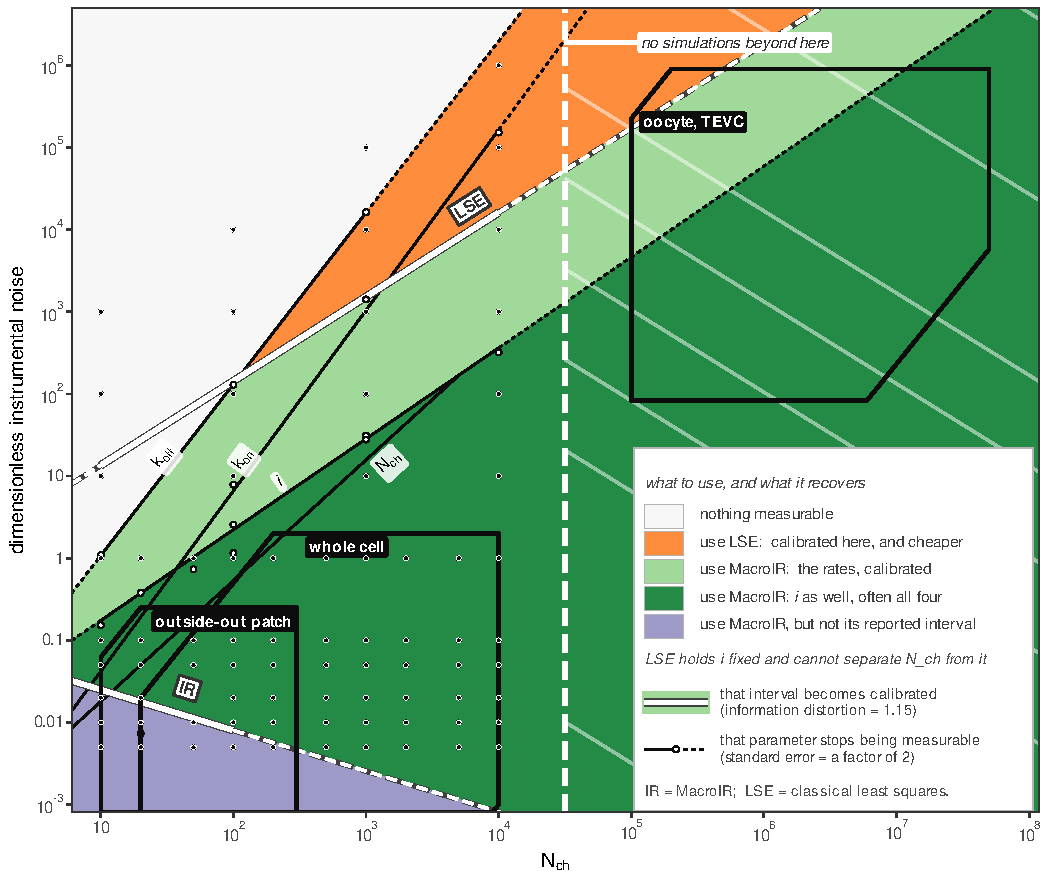
\includegraphics[width=\linewidth]{Figure_7}
\end{fullwidth}
\caption{\textbf{What a macroscopic recording can be asked for, and which method can deliver it.} The design plane, channel number $N_{\mathrm{ch}}$ against dimensionless instrumental noise, at one acquisition interval ($\Delta\!\cdot\!k_{\mathrm{off}}=0.1$). Every cell is filled with which parameters survive there, counting one as recovered when its distortion-corrected standard error is inside a factor of two, and five regions partition the plane, each stated in the key as a recommendation and listed in the key's own vertical order, so that it reads as a section through the map: near-white, where nothing is measurable; amber, where the rates alone survive and classical least squares (\texttt{LSE}) is calibrated there, so the cheaper method is the one to use; pale green, where the rates alone survive but least squares reports an interval that is too narrow; dark green, where the unitary conductance $i$ is recovered as well, with $k_{\mathrm{off}}$ and usually with $k_{\mathrm{on}}$ and $N_{\mathrm{ch}}$; and violet, where the recursive likelihood's own interval (\texttt{IR}) is not calibrated whatever the yield, which overrides. Two classes of line cross the plane and are set differently because they answer different questions: a white line cased in dark, labelled the same way, marks where a method's reported error bar becomes calibrated (information distortion $=1.15$, a $7\%$ error on the reported standard deviation), and a thin black line marks where a parameter stops being measurable. Two of the four black lines carry the partition, those for $i$ and $k_{\mathrm{off}}$; the other two subdivide the dark green region without partitioning it. Each is a power law fitted through the measured crossings, drawn as open dots, with slopes $+1.11$ for $i$, $+1.47$ for $N_{\mathrm{ch}}$, $+2.09$ for $k_{\mathrm{off}}$, $+2.20$ for $k_{\mathrm{on}}$, $+1.03$ for the calibration of least squares and $-0.50$ for that of the likelihood, the one boundary with a negative slope because instrumental noise makes the emission more Gaussian and so repairs the closure. The partition is measured rather than imposed: only six subsets of the four parameters occur in the $80$ cells, they nest at this resolution with no counterexample, and classifying every cell twice, once from its own measurements and once from the fitted lines, $78$ of the $80$ agree, the two failures falling outside the support of the fit that misplaces them. Least squares holds the unitary current fixed and cannot separate the channel count from it, so over the $63$ cells that recover the conductance it has nothing to report about the amplitude at all, which is a property of the method and not a finding about its error bar; where the two do compete, in the $11$ cells recovering the rates alone, its interval is calibrated in $3$, and where it is calibrated it is also no less precise: over the $32$ cells in which both were run the ratio of the distortion-corrected standard error, least squares over the likelihood, has a median of $1.04$ on $k_{\mathrm{off}}$ and $1.01$ on $k_{\mathrm{on}}$, the recursion buying resolution on the rates only where channels are few ($1.89$ at five, $1.11$ at ten, $0.99$ at ten thousand) and buying most of it in the violet corner, at a median of $1.64$, which is the one place its own reported interval has to be corrected first. The key therefore states each region as a recommendation. Filled dots are the simulated cells, $5$ to $10^4$ channels and $0.005$ to $10^6$ in noise; every line is solid only over the channel range in which its own crossings were found and dashed outside it, and past the last simulated column the fills are veiled, so the $56\%$ of the width carrying no cell is visible as such. The noise axis is dimensionless by construction, $\tilde S = \sigma^2/(B\,\tau\,i^2)$ with $\sigma$ the RMS current noise in a bandwidth $B$, $\tau=1/k_{\mathrm{off}}$ and $i$ the unitary current, so that a whole-cell rig at $1$ pA RMS in a $1$ kHz band recording $1$ pA channels with a $10$ ms relaxation sits at $\tilde S = 0.1$; no second axis in picoamps is drawn because the conversion goes as $i^2$, so an axis placed at an assumed $1$ pA would be two decades wrong for a $10$ pA channel, more than the resolution of the map itself. Three recording configurations are placed on the same plane as heavy outlines with reversed tabs: an excised outside-out patch at $10$ to $300$ channels, whole cell at $20$ to $10^4$, and an oocyte under two-electrode voltage clamp (TEVC) at $10^5$ to $5\times10^7$, their channel ranges derived from the smallest and largest current each can hold and their noise ranges from the reported rig-to-rig spread. The map is a concept map and not a phase diagram: loosening the measurability criterion from a factor of two to a factor of ten lifts the four parameter boundaries by a median factor of $9.0$ to $14.4$ in noise and loosening the calibration criterion from $1.15$ to $1.30$ lowers the other two by a factor of $0.50$, which leaves the layout intact and no position better than about a decade. All of it is the two-state scheme at a single open probability and a single concentration-jump protocol.}  % src: projects/eLife_2025/figures/paper_both/Figure_7_caption.md (the long form this compresses) ; figure_7.Rmd chunk `map` (revision AM, 2026-07-31; all boundaries IR-sourced, the predecessor took the rates from least squares which cannot measure k_on) ; subset counts 51/1/11/5/6/6, region counts 54/8/3/9/6, the 78-of-80 confusion table and the criterion sensitivities are measured, not fitted, and printed by the chunk on every render
\label{fig:map}
\end{figure}
